\documentclass[11pt,a4paper]{article}
\usepackage[utf8]{inputenc}
\usepackage[T1]{fontenc}
\hyphenpenalty=10000
\exhyphenpenalty=10000
\emergencystretch=3em
\usepackage{amsmath,amssymb}
\usepackage{booktabs}
\usepackage{tikz}
\usepackage[margin=2.4cm]{geometry}
\usepackage{xcolor}
\usepackage{enumitem}

\definecolor{pA}{RGB}{200,220,245}
\definecolor{pB}{RGB}{255,228,190}
\definecolor{pC}{RGB}{205,235,205}
\definecolor{pD}{RGB}{245,200,200}

\newcommand{\N}{342\,907}
\setlength{\parindent}{0pt}
\setlength{\parskip}{0.55em}

\title{Fatoração por somas posicionais:\\ a forma geométrica}
\date{26 de outubro de 2026}
\author{}

\begin{document}
\maketitle

\noindent Exemplo guia: $N = 877\cdot 391 = \N$. Os fatores só aparecem para conferir a estrutura; o objetivo é entender o que a estrutura diz quando só se conhece $N$.

\section{A identidade e o que ela mede}

Para qualquer base $x$ e fatores $P,Q$ em qualquer ordem, com desvios $a=P-x$ e $b=Q-x$ (podem ser negativos). A distância $d=b-a=Q-P$ não depende da base, e seu sinal diz qual fator é o maior; sem saber a ordem, $d$ fica com sinal livre:
\[
(x+a)(x+b) \;=\; x\,(x+a+b) \;+\; a\,b .
\]
O termo $x+a+b$ é o \emph{cruzamento}: um fator mais o desvio do outro. Ele pode ser escrito de duas formas ($P+b=Q+a$), o que serve de conferência contra erro de escrita. O produto $ab$ é o \emph{resto}. Quando a base está perto dos fatores, $ab$ é pequeno e as duas parcelas não se misturam; quando está longe, $ab$ pesa e as somas se sobrepõem.

Geometricamente é uma tesselação. O retângulo $(x+a)\times(x+b)$ se divide em $x^2$, $xa$, $xb$ e $ab$. As três primeiras peças se reencaixam lado a lado numa faixa de altura $x$ e comprimento $x+a+b$, e sobra o retângulo $ab$ (figura com $x=300$, $a=91$, $b=577$):

\begin{center}
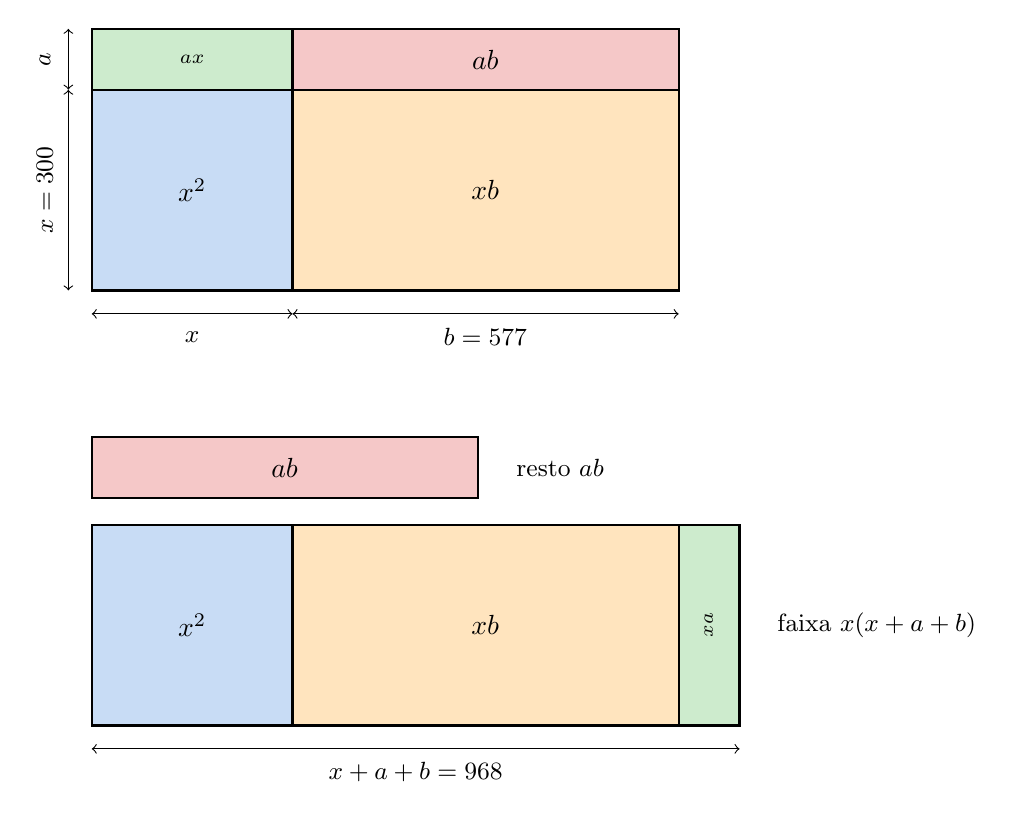
\begin{tikzpicture}[x=0.0085cm,y=0.0085cm]
  % retângulo original, em quatro peças
  \fill[pA] (0,0)   rectangle (300,300);
  \fill[pB] (300,0) rectangle (877,300);
  \fill[pC] (0,300) rectangle (300,391);
  \fill[pD] (300,300) rectangle (877,391);
  \draw[thick] (0,0) rectangle (877,391);
  \draw[thick] (300,0) -- (300,391);
  \draw[thick] (0,300) -- (877,300);
  \node at (150,150) {$x^2$};
  \node at (588,150) {$xb$};
  \node at (150,345) {\scriptsize $ax$};
  \node at (588,345) {$ab$};
  \draw[<->] (0,-35) -- (300,-35);   \node at (150,-70) {\small $x$};
  \draw[<->] (300,-35) -- (877,-35); \node at (588,-70) {\small $b=577$};
  \draw[<->] (-35,0) -- (-35,300);   \node[rotate=90] at (-70,150) {\small $x=300$};
  \draw[<->] (-35,300) -- (-35,391); \node[rotate=90] at (-70,345) {\small $a$};
  % reencaixe: faixa x por (x+a+b) mais o resto ab
  \begin{scope}[shift={(0,-650)}]
    \fill[pA] (0,0)   rectangle (300,300);
    \fill[pB] (300,0) rectangle (877,300);
    \fill[pC] (877,0) rectangle (968,300);
    \draw[thick] (0,0) rectangle (968,300);
    \draw[thick] (300,0) -- (300,300);
    \draw[thick] (877,0) -- (877,300);
    \node at (150,150) {$x^2$};
    \node at (588,150) {$xb$};
    \node[rotate=90] at (922,150) {\scriptsize $xa$};
    \fill[pD] (0,340) rectangle (577,431);
    \draw[thick] (0,340) rectangle (577,431);
    \node at (288,385) {$ab$};
    \node[anchor=west] at (620,385) {\small resto $ab$};
    \node[anchor=west] at (1010,150) {\small faixa $x(x+a+b)$};
    \draw[<->] (0,-35) -- (968,-35); \node at (484,-70) {\small $x+a+b=968$};
  \end{scope}
\end{tikzpicture}
\end{center}

\section{O retângulo em quatro peças}

$N$ é a área de um retângulo $877\times 391$. Cortar os lados em $800+77$ e $300+91$ o divide em quatro peças, cada uma numa escala de posição própria:

\begin{center}
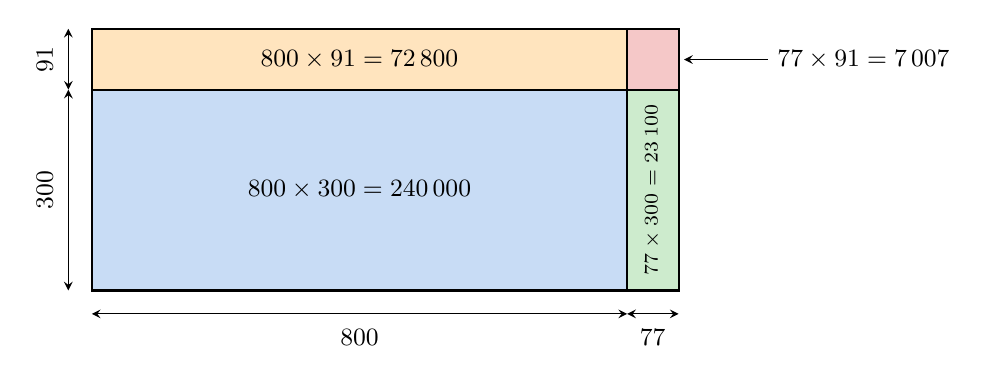
\begin{tikzpicture}[x=0.0085cm,y=0.0085cm,>=stealth]
  % peças
  \fill[pA] (0,0)   rectangle (800,300);
  \fill[pB] (0,300) rectangle (800,391);
  \fill[pC] (800,0) rectangle (877,300);
  \fill[pD] (800,300) rectangle (877,391);
  \draw[thick] (0,0) rectangle (877,391);
  \draw[thick] (800,0) -- (800,391);
  \draw[thick] (0,300) -- (877,300);
  % rótulos das peças
  \node at (400,150) {\small $800\times 300 = 240\,000$};
  \node at (400,345) {\small $800\times 91 = 72\,800$};
  \node[rotate=90] at (838,150) {\scriptsize $77\times 300 = 23\,100$};
  \draw[->] (1010,345) -- (885,345);
  \node[anchor=west] at (1010,345) {\small $77\times 91 = 7\,007$};
  % medidas
  \draw[<->] (0,-35) -- (800,-35); \node at (400,-70) {\small $800$};
  \draw[<->] (800,-35) -- (877,-35); \node at (838,-70) {\small $77$};
  \draw[<->] (-35,0) -- (-35,300); \node[rotate=90] at (-70,150) {\small $300$};
  \draw[<->] (-35,300) -- (-35,391); \node[rotate=90] at (-70,345) {\small $91$};
\end{tikzpicture}
\end{center}

\begin{center}
\begin{tabular}{llr}
\toprule
peça & lados & área \\
\midrule
canto grande (extremo) & $800\times 300$ & $240\,000$ \\
faixa 1 & $800\times 91$ & $72\,800$ \\
faixa 2 & $77\times 300$ & $23\,100$ \\
canto pequeno (resto) & $77\times 91$ & $7\,007$ \\
\midrule
soma & & $\N$ \\
\bottomrule
\end{tabular}
\end{center}

O canto grande é uma tabuada ($3\cdot 8=24$) seguida de zeros. As duas faixas formam o \emph{centro} ($95\,900$, par). O canto pequeno carrega os finais ímpares (o $07$ de $7\,007$). Parte par e parte ímpar ficam em peças diferentes, por isso não há vai-um escondido.

\section{Soma e diferença posicionais}

Chamando de $P$ o menor fator (só um nome, sem perda de generalidade; $Q-P\ge 0$), os blocos e os desvios se combinam, com sinal, assim:
\begin{align*}
Q-P &= (800-300) + (77-91) = 500 - 14 = 486,\\
Q+P &= (800+300) + (77+91) = 1100 + 168 = 1268 .
\end{align*}
Como $|77-91|<10^2$, a diferença fica a menos de um bloco de $k\cdot 10^n$ (aqui $k=5$, $n=2$): $400<486<600$. Os dígitos de $486$ não são coeficientes; ele sai de $5\cdot 100$ menos $14$, com um empréstimo do bloco. E fecha com $N$:
\[
4N = (Q+P)^2-(Q-P)^2 = 1268^2-486^2 = 1\,607\,824-236\,196 = 1\,371\,628 .
\]

\section{Caso equidistante: diferença de quadrados}

Na base média $x=634=(P+Q)/2$ os desvios são $\pm 243$, o cruzamento é a própria base e
\[
N = 634^2 - 243^2 = 401\,956 - 59\,049 = \N .
\]
Geometricamente, o retângulo $877\times 391$ se rearranja num quadrado de lado $634$ sem um quadrado de lado $243$ (um gnômon):

\begin{center}
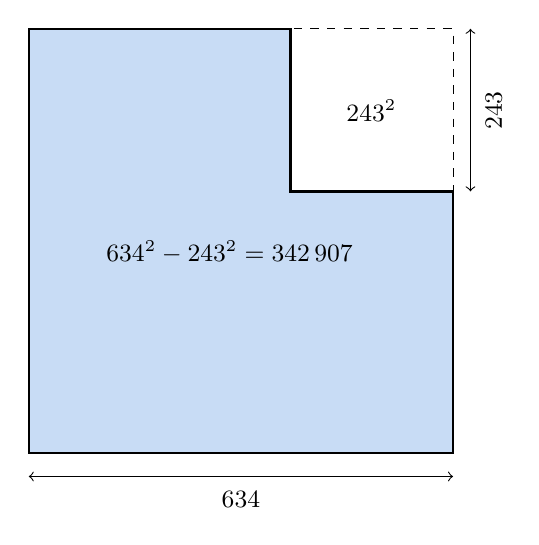
\begin{tikzpicture}[x=0.0085cm,y=0.0085cm]
  \fill[pA] (0,0) rectangle (634,634);
  \fill[white] (391,391) rectangle (634,634);
  \draw[thick] (0,0) -- (634,0) -- (634,391) -- (391,391) -- (391,634) -- (0,634) -- cycle;
  \draw[dashed] (391,391) rectangle (634,634);
  \node at (300,300) {\small $634^2-243^2=\N$};
  \node at (512,512) {\small $243^2$};
  \draw[<->] (0,-35) -- (634,-35); \node at (317,-70) {\small $634$};
  \draw[<->] (660,391) -- (660,634); \node[rotate=90] at (695,512) {\small $243$};
\end{tikzpicture}
\end{center}

Esse é o caso fácil de ler (como $a^2+b^2$). A dificuldade é que a base $634$ só se conhece sabendo os fatores.

\section{Bases próximas e distantes}

Mesmos fatores, várias bases. A coluna $ab/N$ mostra quanto de $N$ fica no resto:

\begin{center}
\begin{tabular}{rrrrrrr}
\toprule
$x$ & $a$ & $b$ & $x+a+b$ & $x(x+a+b)$ & $ab$ & $|ab|/N$ \\
\midrule
0    & 391  & 877  & 1268 & 0       & 342\,907 & 100\% \\
100  & 291  & 777  & 1168 & 116\,800 & 226\,107 & 66\% \\
300  & 91   & 577  & 968  & 290\,400 & 52\,507  & 15\% \\
500  & $-109$ & 377 & 768  & 384\,000 & $-41\,093$ & 12\% \\
634  & $-243$ & 243 & 634  & 401\,956 & $-59\,049$ & 17\% \\
800  & $-409$ & 77  & 468  & 374\,400 & $-31\,493$ & 9\% \\
1000 & $-609$ & $-123$ & 268 & 268\,000 & 74\,907 & 22\% \\
\bottomrule
\end{tabular}
\end{center}

O sinal de $ab$ é positivo antes de $391$, negativo entre $391$ e $877$ e positivo depois de $877$: o desvio zera exatamente em cada fator. Nenhuma base deixa os dois desvios pequenos quando os fatores estão distantes: o menor desvio máximo é $243$, na base $634$.

\section{Forma encadeada e redução do resto sem divisão}

Escrevendo um fator em função do outro, $Q=P+d$ com $P=x+a$ e $d=b-a$ de qualquer sinal ($x=300$, $a=91$, $d=486$):
\[
(x+a)(x+a+d) = x\,(x+2a+d) + a\,(a+d).
\]
Como $b=a+d$, esta é a identidade da seção 1, $(x+a)(x+b)=x(x+a+b)+ab$, com $x+2a+d=x+a+b$ e $a(a+d)=ab$. A escrita só mostra que $b$ contém $a$: o $2a$ é a soma que se repete, pois $a$ entra como desvio do primeiro fator e de novo dentro do segundo. Com os números:
\[
391\cdot 877 = 300\,(300+2\cdot 91+486) + 91\cdot 577 = 300\cdot 968 + 91\cdot 577 .
\]
Conferência das somas (a mesma $P+b=Q+a$ da seção 1): o cruzamento $x+2a+d$ deve ser igual a $P+Q-x$, e de fato $300+182+486 = 968 = 1268-300$.

Se $a+d$ é escrito como $k$ somas de $a$ mais uma sobra $r$, então $a(a+d)=k\,a^2+a\,r$, e o termo $a\,r$ é um produto menor do mesmo tipo. Para $91\cdot 577$ (somando $a$ repetidamente, sem dividir):
\begin{align*}
91\cdot 577 &= 6\cdot 91^2 + 91\cdot 31 = 49\,686 + 2\,821,\\
31\cdot 91  &= 2\cdot 31^2 + 31\cdot 29 = 1\,922 + 899,\\
29\cdot 31  &= 1\cdot 29^2 + 29\cdot 2 = 841 + 58,\\
2\cdot 29   &= 14\cdot 2^2 + 2\cdot 1 = 56 + 2 .
\end{align*}
Total: $52\,507$ $\checkmark$. Os coeficientes $6,2,1,14$ são contagens de somas, não quocientes calculados. A cadeia coincide com o algoritmo de Euclides.

Juntando a forma encadeada com o primeiro passo da redução ($577 = 6\cdot 91+31$):
\[
391\cdot 877 = 300\,(300+2\cdot 91+486) + 6\cdot 91^2 + 31\cdot 91
= 290\,400 + 49\,686 + 2\,821 = \N .
\]

\textbf{Forma da diferença.} Partindo do fator maior, $P=Q-d$ ($391=877-486$). Com $Q=x+b$:
\[
(x+b)(x+b-d) = x\,(x+2b-d) + b\,(b-d).
\]
É a mesma identidade com $a=b-d$: agora é o $b$ que se repete e o resto é $b(b-d)$. Com $x=300$ (aqui $b=577>x$ e $b-d=91$):
\[
877\cdot 391 = 300\,(300+2\cdot 577-486) + 577\cdot 91 = 300\cdot 968 + 52\,507 = \N .
\]
Com $x=800$ (aqui $b=77<x$ e $b-d=-409$, então o resto é negativo):
\[
877\cdot 391 = 800\,(800+2\cdot 77-486) + 77\cdot(-409) = 374\,400 - 31\,493 = \N .
\]
A forma da soma sobe do fator menor ($P+d=Q$) e a da diferença desce do maior ($Q-d=P$). Não é uma identidade nova: é a forma da soma com os papéis trocados, ou com $d<0$. Como a ordem de $P$ e $Q$ não é conhecida de antemão, basta uma fórmula com $d$ de sinal livre. Nas duas, $x+a+b$ é o mesmo cruzamento.

\section{Funil posicional}

Fixando os dígitos dos fatores de cima para baixo (fatores de 3 dígitos, $p\le q$) e mantendo só os pares cujo intervalo contém $N$, sobram:
\begin{center}
\begin{tabular}{lr}
\toprule
nível & pares que sobrevivem \\
\midrule
1 dígito de cada & 7 \\
2 dígitos de cada & 57 \\
3 dígitos (fatores completos) & 1 \\
\bottomrule
\end{tabular}
\end{center}
No nível 1 os pares são $(3,8)$, $(3,9)$, $(4,6)$, $(4,7)$, $(4,8)$, $(5,5)$, $(5,6)$, ou seja, as bases $(300,800)$, $(300,900)$, \ldots. O par certo, $(300,800)$, é um deles. O funil fecha em $(391,877)$, mas o meio é mais largo que o começo.

\section{Pontos em aberto}

\begin{itemize}[leftmargin=1.4em]
  \item \textbf{Resto de $N$ por $x$ não dá direção.} Perto do fator $391$, os restos para $x=386,\dots,396$ são $139,25,303,198,97,0,299,211,127,47,367$. Só zeram exatamente no fator (correlação entre distância ao fator e resto: $-0{,}015$). Testar ``dá zero?'' com o resto é divisão de tentativa.
  \item \textbf{O sinal de $ab$ muda nos fatores}, mas calculá-lo exige os fatores. Falta uma grandeza obtida só de $N$ e da base que acompanhe esse sinal ou encolha ao se aproximar de um fator.
  \item \textbf{Escolha do corte.} Dos 7 pares do nível 1 (cada um define janelas para $Q+P$ e $Q-P$ de largura menor que $10^n$), falta o critério que seleciona $k$ e o sinal do empréstimo.
  \item \textbf{Casas baixas.} Vale $ab\equiv N \pmod{100}$ ($7007\equiv 7$) e os finais dos fatores estão em $\{1,3,7,9\}$ quando $N$ é ímpar sem fator $5$. Cruzar esse corte com o intervalo ainda não foi testado.
  \item \textbf{Escala.} As contagens acima são de um único $N$ de seis dígitos; não foi medido como o meio do funil cresce para números maiores.
\end{itemize}

\end{document}
